\documentclass{beamer} % Article for most documents; beamer for presentations.

% Packages loaded
\usepackage[utf8]{inputenc} % Loaded by default in Overleaf
\usepackage{graphicx} % For pictures
\usepackage{amsmath} % For math
\usepackage{url} % For URLs. Another alternative is the package href, which allows embedded hyperlinks in text.

% Defining new theorems: \newtheorem{local name of environment}{displayed name of environment}
\newtheorem{idea}{Big Ideas!}
% In order words, we will type \begin{idea} to make a theorem environment labelled "Big Ideas!"

% Title meta-data
\title{MATH340 Day 6}
\author{Zane and Dr. McNelis}
\date{30, August 2019}

% Today: beamer, new theorems, more \left \right, labels/refs, footnotes, \text{}, \url{}, Richard Hamming's Plaid Suit.

\begin{document}

\maketitle % In beamer, this makes its own slide for free.

\begin{frame}{Outline}
    \tableofcontents % You will never guess what this command does.
    % (It generates a table of contents based on the sections/subsections/subsubsections you have. You can specify the "depth" additionally, but you have to look up how.
    % You can do a list of figures and tables as well, and also an index. If you need these, you can find the documentation on wikibooks/CTAN/google.
\end{frame}

\section{Introduction}

% For every "slide" you want in your presentation, you need to have a new frame environment. This frame environment has text and a picture in it.
% The second argument to \begin{frame}{this one} will change the title of the slide.
\begin{frame}{Why Chocolate Is Good}
% Everything inside the frame will be on the same slide.
    I love chocolate!
    \begin{figure} % We already learned figures, so I will not explain this.
        \centering
        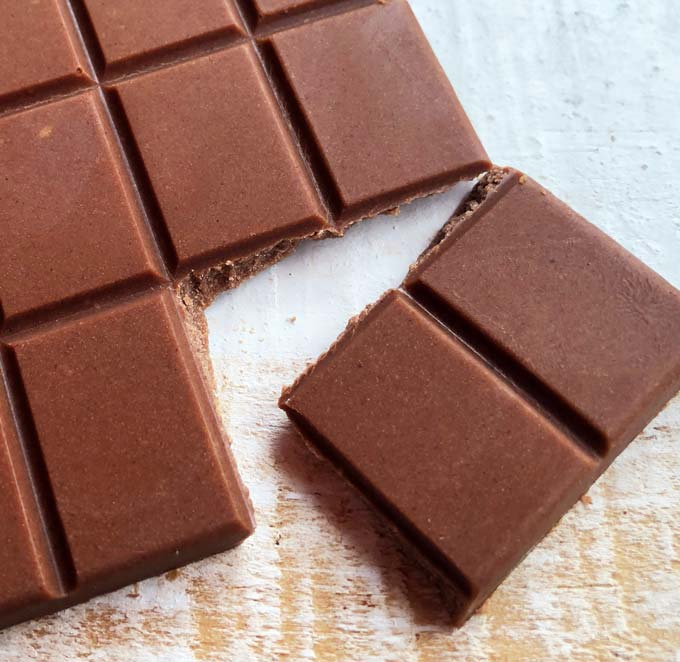
\includegraphics[width=0.5\textwidth]{my_image.jpg}
        \caption{(This is chocolate.)}
        \label{fig:chocolate} % This assigns a nickname to the figure so we can reference it later without remembering the number.
    \end{figure}
\end{frame}

\subsection{Some Big Ideas}

\begin{frame}{Free Chocolate for Everyone}
    % This is how we use the new idea environment that we defined.
    Dr. McNelis thinks she has a good idea.
    \begin{idea}[Free Chocolate]
    Chocolate makes people happy. The government should send us a piece of chocolate every day. (Elections will be much better.)
    \end{idea}
    % The optional argument after \begin{idea} will let us give a name to our big idea.
\end{frame}

% How to do pauses
\begin{frame}{Another Big Idea}
% The angle brackets next to the items below will tell your presentation which slides these items should show up on. Think about this like powerpoint animations.
    List of types of chocolate:
    \begin{enumerate} % We know how to do lists.
        \item<1-> Dark chocolate 
        \item<2-3> Milk chocolate
        \item<3-5> White chocolate
        \item<2-> Dutch prepared chocolate
        \item<4-> Bittersweet
        \item<5-> German chocolate
    \end{enumerate}
\end{frame}

\begin{frame}{WE NEED PROOF!}
\[ \text{Which type(day)} = \left\{ % Recall {} are reserved characters in LaTeX. \{ \} prints the brace.
\begin{array}{ll}
     \text{milk} & \text{if day} \in \{M,W,F\} \\
     \text{dark} & \text{if day} \in \{T, Th\} \\
     \text{bittersweet} & \text{if day} \in \{S, Su\}
\end{array}
\right. \]
% Explanations:
% If you want an asymmetrical delimiter in left/right, you can use a period (e.g. as above) instead of the delimiter you don't want. You CANNOT just use \left or \right alone, they must be paired.
% \in prints the "element of" symbol.
% \text allows you to type regular words in math environments and not have them be ugly.
\end{frame}

% References

\begin{frame}{Frame Title}
    "The purpose of computation is insight, not numbers." - Richard Hamming\footnote{Richard Hamming was a famous mathematician, so you should listen to him. \url{https://en.wikipedia.org/wiki/Richard_Hamming} }
    
    You should also look at Figure \ref{fig:chocolate}. % Use the \ref{} command to put the figure number in the text. This grabs the number associated with the picture's nickname.
\end{frame}

% The command \footnote{} will make a footnote at the bottom of the current page or slide.

\end{document}
